\documentclass{beamer}[10]

\usepackage{graphicx}
\usepackage{xcolor}
\usepackage{tabto}
%\usepackage{beamerthemesplit}
\usepackage{tikz}
\usepackage{cancel}
\usepackage{verbatim}
\usepackage{fancybox}
\usepackage{enumerate}
\usepackage{amsmath,amssymb,amsthm,textcomp,mathtools}
\usepackage[super]{nth}
\usepackage[amssymb]{SIunits}
\usepackage{booktabs}
\usepackage{cancel}
\usepackage{bm}
\usepackage[utf8]{inputenc}
\usepackage{tabularx}
\usepackage{ragged2e}
\newcolumntype{Y}{ >{\RaggedRight\arraybackslash}X}
\usetikzlibrary{arrows,shapes}
\newcommand\T{\rule{0pt}{2.6ex}}
\newcommand\B{\rule[-1.2ex]{0pt}{0pt}}
\definecolor{UUcrimson}{RGB}{204,0,0}
\mode<presentation>
{ \usetheme{default}
  \usecolortheme[named=UUcrimson]{structure}
  \useinnertheme{circles}
  \setbeamercovered{transparent}
  \setbeamertemplate{blocks}[rounded]
  \usefonttheme[onlymath]{serif}
  \setbeamertemplate{navigation symbols}{}
  \setbeamertemplate{footline}[page number]
  \setbeamertemplate{navigation symbols}{}
  \setbeamercolor{section in toc}{fg=black,bg=white}
  \setbeamercolor{alerted text}{fg=UUcrimson!80!gray}
  \setbeamercolor*{palette primary}{fg=white,bg=UUcrimson}
  \setbeamercolor*{palette secondary}{fg=UUcrimson!70!black,bg=gray!15!white}
  \setbeamercolor*{palette tertiary}{bg=UUcrimson!80!black,fg=gray!10!white}
  \setbeamercolor*{palette quaternary}{fg=UUcrimson,bg=gray!5!white}
  \setbeamercolor*{palette sidebar primary}{fg=UUcrimson!10!black}
  \setbeamercolor*{palette sidebar secondary}{fg=white}
  \setbeamercolor*{palette sidebar tertiary}{fg=UUcrimson!50!black}
  \setbeamercolor*{palette sidebar quaternary}{fg=gray!10!white}
  \setbeamercolor{titlelike}{parent=palette primary,fg=white}
  \setbeamercolor{frametitle}{bg=UUcrimson}
  \setbeamercolor{frametitle right}{bg=UUcrimson}
  \setbeamercolor*{separation line}{}
  \setbeamercolor*{fine separation line}{}
}

\usetikzlibrary{backgrounds}
\makeatletter
\tikzstyle{every picture}+=[remember picture]
\tikzset{%
  fancy quotes/.style={
    text width=\fq@width pt,
    align=justify,
    inner sep=1em,
    anchor=north west,
    minimum width=\linewidth,
    font=\itshape
  },
  fancy quotes width/.initial={.8\linewidth},
  fancy quotes marks/.style={
    scale=8,
    text=white,
    inner sep=0pt,
  },
  fancy quotes opening/.style={
    fancy quotes marks,
  },
  fancy quotes closing/.style={
    fancy quotes marks,
  },
  fancy quotes background/.style={
    show background rectangle,
    inner frame xsep=0pt,
    background rectangle/.style={
      fill=gray!25,
      rounded corners,
    },
  }
}
\newenvironment{fancyquotes}[1][]{%
\noindent
\tikzpicture[fancy quotes background]
\node[fancy quotes opening,anchor=north west] (fq@ul) at (0,0) {``};
\tikz@scan@one@point\pgfutil@firstofone(fq@ul.east)
\pgfmathsetmacro{\fq@width}{\linewidth - 2*\pgf@x}
\node[fancy quotes,#1] (fq@txt) at (fq@ul.north west) \bgroup}
{\egroup;
\node[overlay,fancy quotes closing,anchor=east] at (fq@txt.south east) {''};
\endtikzpicture}
\makeatother


\usetikzlibrary{backgrounds}
\makeatletter
\tikzstyle{every picture}+=[remember picture]
\tikzset{%
  fancy defs/.style={
    text width=\fq@width pt,
    align=justify,
    inner sep=0.25em,
    anchor=north west,
    minimum width=\linewidth,
    font=\itshape
  },
  fancy defs width/.initial={.8\linewidth},
  fancy defs marks/.style={
    scale=8,
    text=white,
    inner sep=0pt,
  },
  fancy defs opening/.style={
    fancy defs marks,
  },
  fancy defs closing/.style={
    fancy defs marks,
  },
  fancy defs background/.style={
    show background rectangle,
    inner frame xsep=0pt,
    background rectangle/.style={
      fill=gray!25,
      rounded corners,
    },
  }
}
\newenvironment{fancydefs}[1][]{%
\noindent
\tikzpicture[fancy defs background]
\node[fancy defs opening,anchor=north west] (fq@ul) at (0,0) {};
\tikz@scan@one@point\pgfutil@firstofone(fq@ul.east)
\pgfmathsetmacro{\fq@width}{\linewidth - 2*\pgf@x}
\node[fancy defs,#1] (fq@txt) at (fq@ul.north west) \bgroup}
{\egroup;
\node[overlay,fancy defs closing,anchor=east] at (fq@txt.south east) {};
\endtikzpicture}
\makeatother
\usepackage{scalerel}[2014/03/10]
\usepackage{stackengine}
\usepackage{empheq}
\newcommand*\widefbox[1]{\fbox{\hspace{0.5em}#1\hspace{0.5em}}}

\newcommand\reallywidetilde[1]{\ThisStyle{%
  \setbox0=\hbox{$\SavedStyle#1$}%
  \stackengine{-.1\LMpt}{$\SavedStyle#1$}{%
    \stretchto{\scaleto{\SavedStyle\mkern.2mu\sim}{.5467\wd0}}{.4\ht0}%
%    .2mu is the kern imbalance when clipping white space
%    .5467++++ is \ht/[kerned \wd] aspect ratio for \sim glyph
  }{O}{c}{F}{T}{S}%
}}
\usepackage{media9}

\logo{
\includegraphics[width=0.75cm]{logo.jpg}}
\author[Gibbs]{Dr. Jeremy A. Gibbs}
\institute{Department of Mechanical Engineering\\University of Utah}
\date{Spring 2017}
\title{Environmental Fluid Dynamics: Lecture 14}
% colors
\newcommand{\ihat}{\boldsymbol{\hat{\imath}}}
\newcommand{\jhat}{\boldsymbol{\hat{\jmath}}}
\newcommand{\khat}{\boldsymbol{\hat{k}}}
\definecolor{colororange}{HTML}{E65100} % orange
\definecolor{colordgray}{HTML}{795548} % dark gray for note
\definecolor{colorhgray}{HTML}{212121} % heavy dark gray for normal text
\definecolor{colorgreen}{HTML}{009688} % green
\definecolor{colorwhite}{HTML}{FFFFFF} % background white
\definecolor{colorlgray}{HTML}{F5F3EE} % background light gray
\definecolor{colorblue}{HTML}{0277BB} % blue
\definecolor{colorred}{HTML}{CC0000} % red
\newcommand{\fontsizeone}{1.9em}
\usepackage{esvect}
\setbeamertemplate{caption}{\raggedright\insertcaption\par}
\newcommand{\framecard}[2][colorgreen]{
  {\setbeamercolor{background canvas}{bg=#1}
    \begin{frame}[plain]
    \vfill
    \begin{center}
     {#2}
    \end{center}
    \vfill
    \end{frame}
  }
}
\begin{document}

%----------------------------------------------------------------------------------------
%	TITLE & TOC SLIDES
%----------------------------------------------------------------------------------------

\begin{frame} 
  \titlepage
\end{frame}

%------------------------------------------------

\begin{frame}
\frametitle{Overview}
\tableofcontents
\end{frame}

%------------------------------------------------
\section{Atmospheric Dynamics: Basic Equations} %
%------------------------------------------------
\subsection{Summation Review}
%------------------------------------------------
\framecard[colorred]{{\color{white}\Huge Summation Review}}
%------------------------------------------------
\begin{frame}{Einstein Summation Review}

Consider:
\begin{align*}
U_m &\Rightarrow \text{generic velocity vector}\\
x_m &\Rightarrow \text{generic component of distance}\\
e_m &\Rightarrow \text{generic unit vector}
\end{align*}
where $m=1,2,3$. We can write the individual components as:
\begin{align*}
U_1 &= u & x_1 &= x & e_1 &= \hat i	\\
U_2 &= v & x_2 &= x & e_2 &= \hat j\\
U_3 &= w & x_3 &= x & e_3 &= \hat k
\end{align*}
A variable with: 
\begin{itemize}
	\item no free indices is a \textbf{scalar}.
	\item one free indice is a \textbf{vector}.
	\item two free indices is a \textbf{tensor}.
\end{itemize}
\end{frame}
%------------------------------------------------
\begin{frame}{Einstein Summation Review}


There are two primary summation operators that we will use:
\begin{itemize}
	\item \textbf{Kronecker Delta}
	$$\delta_{mn} = 
	\begin{cases}
    +1, & \text{if } m=n\\
    0   & \text{if } m \neq n
	\end{cases}$$
	
	\item \textbf{Levi-Civita (Alternating Unit) Tensor}
	$$\epsilon_{mnq} = 
	\begin{cases}
    +1, & \text{if } mnq = 123, 231, 312\quad \text{even permutation}\\
    -1  & \text{if } mnq = 321, 213, 132\quad \text{odd permutation}\\
    0   & \text{if } m=n, n=q, q=m\quad \text{any two indices repeated}
	\end{cases}$$
\end{itemize}
\end{frame}
%------------------------------------------------
\subsection{Mechanical Energy Equation}
%------------------------------------------------
\framecard[colorred]{{\color{white}\Huge Atmospheric Dynamics:\\~\\Mechanical Energy Equation}}
%------------------------------------------------
\begin{frame}{Mechanical Energy Equation}
\begin{itemize}
	\item The mechanical energy equation describes the rate of change of a fluid element's kinetic energy.
	\item To start, we take the dot product of the velocity vector with our momentum balance equation.
	$$\vv{U} \cdot \Bigg(\underbrace{\vphantom{-\frac{1}{\rho}\vv{\nabla}p}\rho\frac{D\vv{U}}{Dt}}_{1} = \underbrace{\vphantom{-\frac{1}{\rho}\vv{\nabla}p}-\vv{\nabla}p}_{2} - \underbrace{\vphantom{-\frac{1}{\rho}\vv{\nabla}p}2\rho\vv{\Omega}\times \vv{U}}_{3} + \underbrace{\vphantom{-\frac{1}{\rho}\vv{\nabla}p}\rho\vv{g}}_{4} + \underbrace{\vphantom{-\frac{1}{\rho}\vv{\nabla}p}\mu \vv{\nabla}^2\vv{U}}_{5}\Bigg)$$
	\item Note: We've multiplied the momentum balance equation by $\rho$
	\item We will examine each term separately and then put together for our final expression.
\end{itemize}
\end{frame}
%------------------------------------------------
\begin{frame}{Mechanical Energy Equation}
\textbf{Term 1}
\begin{align*}
	\vv{U} \cdot \rho\frac{D\vv{U}}{Dt} &= u_i\left(\rho\frac{\partial u_i}{\partial t} + \rho u_j \frac{\partial u_i}{\partial x_j}\right)\\
	&= \rho u_i \frac{\partial u_i}{\partial t} + \rho u_j u_i\frac{\partial u_i}{\partial x_j} \quad \text{use product rule}\\
	&= \rho \frac{\partial \Big(\cfrac{u_i u_i}{2}\Big)}{\partial t} + \rho u_j \frac{\partial \Big(\cfrac{u_i u_i}{2}\Big)}{\partial x_j}\\
	\Aboxed{&= \rho \frac{\partial E}{\partial t} + \rho u_j\frac{\partial E}{\partial x_j}}
\end{align*}
where $E = u_i^2/2$ is kinetic energy.
\end{frame}
%------------------------------------------------
\begin{frame}{Mechanical Energy Equation}
\textbf{Term 2}
\begin{align*}
	\vv{U} \cdot \Big(-\vv{\nabla}p\Big) &= -u_i\frac{\partial p}{\partial x_i}\quad \text{use product rule}\\
	&=-\left(\frac{\partial (pu_i)}{\partial x_i} + p\cancelto{}{\frac{\partial u_i}{\partial x_i}}\right)\\
	\Aboxed{&=-\frac{\partial (pu_i)}{\partial x_i}}
\end{align*}
\end{frame}
%------------------------------------------------
\begin{frame}{Mechanical Energy Equation}
\textbf{Term 3}
$$\vv{U} \cdot \left(-2 \rho\vv{\Omega} \times \vv{U} \right)$$
Recall that the Coriolis has the following components:
\begin{itemize}
	\item $x$: fv
	\item $y$: -fu
	\item $z$: 0
\end{itemize}
This corresponds to $\epsilon_{ij3}fu_j$. So,
$$\vv{U} \cdot \left(-2\rho \vv{\Omega} \times \vv{U} \right) = \boxed{\epsilon_{ij3}fu_iu_j}$$
However, using the rules of the alternating unit tensor, you can show this is equal to zero. Alternatively, you know $-2\rho\Omega\times \vv{U}$ is $\perp$ to $\vv{U}$. Thus, their dot product is zero. Why? 
~\\~\\
Coriolis force does no work!
\end{frame}
%------------------------------------------------
\begin{frame}{Mechanical Energy Equation}
\textbf{Term 4}
$$\vv{U} \cdot \vv{g} = u_i g_i$$
But if we assume that gravity only acts in the $\hat k$ direction, then we can make use of the Kronecker delta:
$$\vv{U} \cdot \rho \vv{g}=  \boxed{\rho u_i g_i \delta_{i3}}$$
\end{frame}
%------------------------------------------------
\begin{frame}{Mechanical Energy Equation}
\textbf{Term 5}
\begin{align*}
\vv{U} \cdot \nu \vv{\nabla}^2\vv{U} &= \mu u_i \frac{\partial^2u_i}{\partial x_j^2}\\
&= \mu u_i \frac{\partial}{\partial x_j}\frac{\partial u_i}{\partial x_j}\\
\Aboxed{&= u_i\frac{\partial \tau_{ij}}{\partial x_j}}
\end{align*}
\end{frame}
%------------------------------------------------
\begin{frame}{Mechanical Energy Equation}
\textbf{All Together}
$$
\underbrace{\vphantom{-\frac{1}{\rho}\vv{\nabla}p}\rho \frac{\partial E}{\partial t}}_{1} + \underbrace{\vphantom{-\frac{1}{\rho}\vv{\nabla}p}\rho u_j\frac{\partial E}{\partial x_j}}_{2}= \underbrace{\vphantom{-\frac{1}{\rho}\vv{\nabla}p}-\frac{\partial (pu_i)}{\partial x_i}}_{3} + \underbrace{\vphantom{-\frac{1}{\rho}\vv{\nabla}p}\rho u_i g_i \delta_{i3}}_{4} + \underbrace{\vphantom{-\frac{1}{\rho}\vv{\nabla}p}u_i\frac{\partial \tau_{ij}}{\partial x_j}}_{5}$$
\textbf{Terms}
\begin{enumerate}
	\item Storage of kinetic energy
	\item Advection of kinetic energy by the bulk flow
	\item Work done against gravity
	\item Work done against viscous forces
\end{enumerate}
\end{frame}
%------------------------------------------------
\begin{frame}{Mechanical Energy Equation}

\begin{itemize}
	\item Note: we can expand the viscous dissipation term as:
	\begin{align*}
	u_i\frac{\partial \tau_{ij}}{\partial x_j} &= \frac{\partial u_i \tau_{ij}}{\partial x_j} - \tau_{ij}\frac{\partial u_i}{\partial x_j}\\
	&=\frac{\partial u_i \tau_{ij}}{\partial x_j} - \tau_{ij}S_{ij}
	\end{align*}
	where $S_{ij}$ is the symmetric part of the velocity gradient.
	\item The first term is the total rate of work, or molecular diffusion.
	\item The second term is the deformation work, or viscous dissipation.
\end{itemize}
\end{frame}
%------------------------------------------------
\subsection{Thermal Energy Equation}
%------------------------------------------------
\framecard[colorred]{{\color{white}\Huge Atmospheric Dynamics:\\~\\Thermal Energy Equation}}
%------------------------------------------------
\begin{frame}{Thermal Energy Equation}

\begin{itemize}
	\item We can write the \nth{1} Law of Thermodynamics for an open unsteady system in words as follows, where total energy = internal ($I$) + kinetic ($E=V^2/2$): 
	\begin{align*}
	\Bigg \{\underbrace{\parbox{6em}{\centering rate of\\ total energy\\accumulation}}_{1}\Bigg\} &= \Bigg \{\underbrace{\parbox{6em}{\centering net rate of\\total energy in\\by advection}}_{2}\Bigg \} + \Bigg \{\underbrace{\parbox{6em}{\centering net rate of\\heat added by\\conduction}}_{3}\Bigg \} \\&+ \Bigg \{\underbrace{\parbox{6em}{\centering net rate of\\heat added by\\radiation}}_{4}\Bigg \} + \Bigg \{\underbrace{\parbox{6em}{\centering net rate of\\heat added by\\phase change}}_{5}\Bigg \}\\
    &- \Bigg \{\underbrace{\parbox{6em}{\centering net rate of\\work done by\\fluid on surroundings}}_{6}\Bigg \}
	\end{align*}
\end{itemize}
\end{frame}
%------------------------------------------------
\begin{frame}{Thermal Energy Equation}

\begin{itemize}
	\item This is seen visually as:
	\begin{figure}
		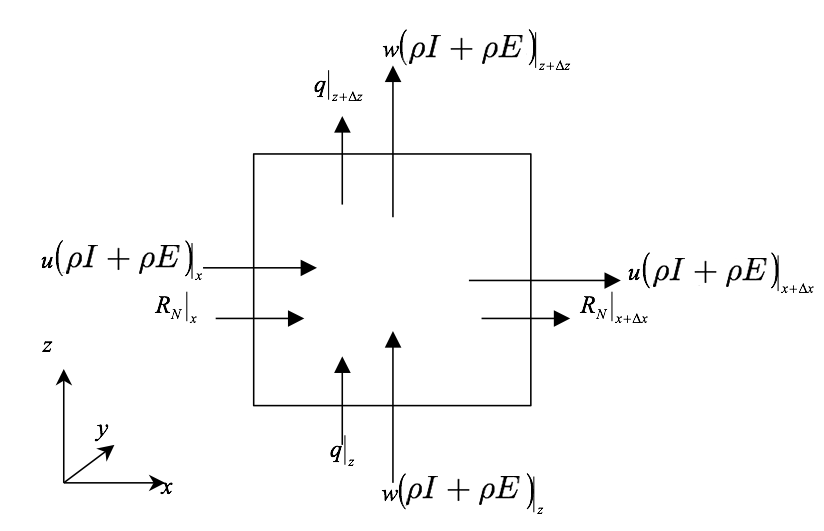
\includegraphics[width=0.9\textwidth]{thermo1}
	\end{figure}
	Let's look separately at each term in the previous description.
\end{itemize}
\end{frame}
%------------------------------------------------
\begin{frame}{Thermal Energy Equation}

\textbf{Term 1}
\begin{itemize}
	\item Rate of accumulation of internal energy per unit volume and kinetic energy within the element (these are in units of $\watt$):
	$$\Delta x \Delta y \Delta z \frac{\partial}{\partial t}(\rho I + \rho E)$$
\end{itemize}
\end{frame}
%------------------------------------------------
\begin{frame}{Thermal Energy Equation}

\textbf{Term 2}
\begin{itemize}
	\item Net rate of advection of internal and kinetic Energy into the volume element:
	\begin{align*}
		&\Delta y\Delta z \left\{u(\rho I + \rho E)_{x+\Delta x} - u(\rho I + \rho E)_{x} \right\} \\
		+ &\Delta x \Delta z\left\{v(\rho I + \rho E)_{y+\Delta y} - v(\rho I + \rho E)_{y} \right\}\\
		+ &\Delta x \Delta y\left\{w(\rho I + \rho E)_{z+\Delta z} - w(\rho I + \rho E)_{z} \right\}
	\end{align*}
\end{itemize}
\end{frame}
%------------------------------------------------
\begin{frame}{Thermal Energy Equation}

\textbf{Term 3}
\begin{itemize}
	\item Net rate of energy input by conduction into the volume element (molecular):
	\begin{align*}
		\Delta y\Delta z (q_x|_x - q_x|_{x+\Delta x}) &+ \Delta x\Delta z (q_y|_y - q_y|_{y+\Delta y}) \\&+ \Delta x\Delta y (q_z|_z - q_z|_{z+\Delta z})
	\end{align*}
\end{itemize}
\end{frame}
%------------------------------------------------
\begin{frame}{Thermal Energy Equation}

\textbf{Term 4}
\begin{itemize}
	\item Net rate of energy input by all wavelengths of radiation into the volume element:
	\begin{align*}
		\Delta y\Delta z (R_{nx}|_x - R_{nx}|_{x+\Delta x}) &+ \Delta x\Delta z (R_{ny}|_y - R_{ny}|_{y+\Delta y}) \\&+ \Delta x\Delta y (R_{nz}|_z - R_{nz}|_{z+\Delta z})
	\end{align*}
\end{itemize}
\end{frame}
%------------------------------------------------
\begin{frame}{Thermal Energy Equation}

\textbf{Term 5}
\begin{itemize}
	\item Net rate of energy input by phase change into the volume element:
	$$\Delta x \Delta y \Delta z (L_v \epsilon)$$
	where $L_v(\sim 2.45\times 10^{6}\ \joule\ \kilo\reciprocal\gram)$ is the latent heat of vaporization/condensation and $\epsilon (\kilo\gram\ \metre\rpcubed\ \reciprocal\second)$ is the evaporation/condensation rate per unit volume.
	\item Note: this is a body sink/source term.
\end{itemize}
\end{frame}
%------------------------------------------------
\begin{frame}{Thermal Energy Equation}

\textbf{Term 6}
\begin{itemize}
	\item Net rate of work done by the fluid element against the surroundings.
	\item Recall that work rate done by a force is the magnitude of the force multiplied by the velocity in the direction of the force:
	$$\dot{W} = \vv{F}\cdot \vv{U}$$
	So we will write the work rates as forces multiplied by velocities acting on our fluid element.
	\item The net rate of work will broken into work against body forces and work against surface forces.
\end{itemize}
\end{frame}
%------------------------------------------------
\begin{frame}{Thermal Energy Equation}

\textbf{Term 6}
\begin{itemize}
	\item Work against body forces: rate of doing work against the gravitational force
	$$\Delta x \Delta y \Delta z (\rho ug_x + \rho vg_y + \rho w g_z)$$
	\item Work against surface forces: rate of doing work against the pressure at the six faces of a volume element
	\begin{align*}
		\Delta y\Delta z \{(pu)_x|_{x+\Delta x} - (pu)_x|_x\} &+ \Delta x\Delta z \{(pv)_y|_{y+\Delta y} - (pv)_y|_y\} \\&+ \Delta x\Delta y \{(pw)_z|_{z+\Delta z} - (pw)_z|_z\}
	\end{align*}
	Note that here we take the work rate to be $(p\cdot\vv{n}dA)\cdot\vv{U}$ where $\vv{n}$ is the outwardly pointing normal vector from the fluid element.
\end{itemize}
\end{frame}
%------------------------------------------------
\begin{frame}{Thermal Energy Equation}

\textbf{Term 6}
\begin{itemize}
	\item Work against surface forces: rate of doing work against the viscous force
	\begin{figure}
	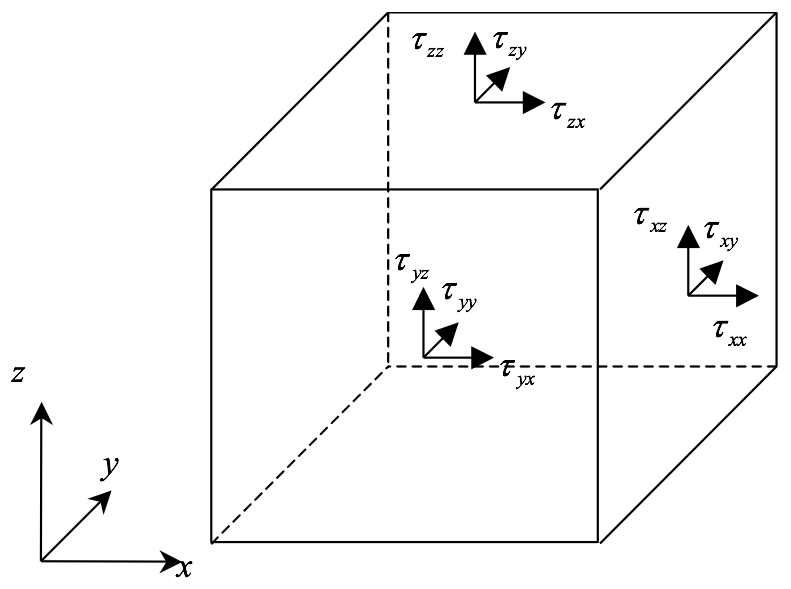
\includegraphics[width=0.8\textwidth]{thermo2}	
	\end{figure}

\end{itemize}
\end{frame}
%------------------------------------------------
\begin{frame}{Thermal Energy Equation}

\textbf{Term 6}
\begin{itemize}
	\item Work against surface forces: rate of doing work against the viscous force
	\begin{align*}
		&\Delta y\Delta z \{ (\tau_{xx}u + \tau_{xy}v + \tau_{xz} w)_{x} - (\tau_{xx}u + \tau_{xy}v + \tau_{xz} w)_{x+\Delta x}\}\\
		+&\Delta x\Delta z \{ (\tau_{yx}u + \tau_{yy}v + \tau_{yz} w)_{y} - (\tau_{yx}u + \tau_{yy}v + \tau_{yz} w)_{y+\Delta y}\}\\
		+&\Delta x\Delta y \{ (\tau_{zx}u + \tau_{zy}v + \tau_{zz} w)_{z} - (\tau_{zx}u + \tau_{zy}v + \tau_{zz} w)_{z+\Delta z}\}
	\end{align*}
\end{itemize}
\end{frame}
%------------------------------------------------
\begin{frame}{Thermal Energy Equation}

\textbf{All Together}
\begin{itemize}
	\item Now we combine all terms, divide by $\Delta x \delta y \Delta z$, and take the limit as $\Delta x \rightarrow 0$, $\Delta y \rightarrow 0$, and $\Delta z \rightarrow 0$ to obtain the \textbf{complete energy equation}:
	\small
	\begin{align*}
		\frac{\partial (\rho I + \rho E)}{\partial t} = &-\left(u\frac{\partial (\rho I + \rho E)}{\partial x} + v\frac{\partial (\rho I + \rho E)}{\partial y} + w\frac{\partial (\rho I + \rho E)}{\partial z}\right)\\
		&-\left(\frac{\partial q_x}{\partial x} + \frac{\partial q_y}{\partial y} + \frac{\partial q_x}{\partial z}\right)-\left(\frac{\partial pu}{\partial x} + \frac{\partial pv}{\partial y} + \frac{\partial pw}{\partial z}\right)\\
		&-\left(\frac{\partial R_{nx}}{\partial x} + \frac{\partial R_{ny}}{\partial y} + \frac{\partial R_{nz}}{\partial z}\right) -\left(\frac{\partial ug_x}{\partial x} + \frac{\partial vg_y}{\partial y} + \frac{\partial wg_z}{\partial z}\right)\\
		&- L_v\epsilon \\
		&-\left\{\frac{\partial (\tau_{xx} u + \tau_{yx} v + \tau_{zx} w)}{\partial x}+\frac{\partial (\tau_{xy} u + \tau_{yy} v + \tau_{zy} w)}{\partial y} \right. \\ &\quad+  \left. \frac{\partial (\tau_{xz} u + \tau_{yz} v + \tau_{zz} w)}{\partial z} \right\}
	\end{align*}
\end{itemize}
\end{frame}
%------------------------------------------------
\begin{frame}{Thermal Energy Equation}

\textbf{All Together}
\begin{itemize}
	\item As with the derivation of the momentum equation, we can utilize Newtonian expressions to relate the velocity gradients and stresses, namely:
	\begin{align*}
	\tau_{xx} &= -2\mu\frac{\partial u}{\partial x} + \frac{2}{3}\mu(\vv{\nabla}\cdot\vv{U}) \qquad \tau_{xy} = \tau_{yx} = -\mu\left(\frac{\partial u}{\partial y} + \frac{\partial v}{\partial x}\right)\\
	\tau_{yy} &= -2\mu\frac{\partial v}{\partial y} + \frac{2}{3}\mu(\vv{\nabla}\cdot\vv{U}) \qquad \tau_{xz} = \tau_{zx} = -\mu\left(\frac{\partial u}{\partial z} + \frac{\partial w}{\partial x}\right)\\
	\tau_{zz} &= -2\mu\frac{\partial w}{\partial z} + \frac{2}{3}\mu(\vv{\nabla}\cdot\vv{U}) \qquad \tau_{zy} = \tau_{yz} = -\mu\left(\frac{\partial w}{\partial y} + \frac{\partial v}{\partial z}\right)\\
	\end{align*}
	Or more compactly:
	$$\tau_{ij} = -2\mu S_{ij} + \frac{2}{3}\mu(\vv{\nabla} \cdot \vv{U}) \delta_{ij}$$
\end{itemize}
\end{frame}
%------------------------------------------------
\begin{frame}{Thermal Energy Equation}

\textbf{All Together}
\begin{itemize}
	\item We now subtract the $E$ equation (slide 13) from the complete energy equation to yield the \textbf{thermal energy equation}:
	$$\underbrace{\rho \frac{DI}{Dt}}_{1} = \underbrace{\vphantom{\frac{DI}{Dt}}-\vv{\nabla}\cdot \vv{q}}_{2} -\underbrace{\vphantom{\frac{DI}{Dt}}\vv{\nabla}\cdot (p\vv{U})}_{3} \underbrace{\vphantom{\frac{DI}{Dt}}-\vv{\nabla}\cdot \vv{R_n}}_{4} + \underbrace{\vphantom{\frac{DI}{Dt}}L_v\epsilon}_{5} + \underbrace{\vphantom{\frac{DI}{Dt}}\mu \Phi_\nu}_{6}$$
\end{itemize}
\textbf{Terms (per unit volume)}
\begin{enumerate}
	\item Rate of gain of internal energy
	\item Rate of internal energy input by conduction
	\item Reversible rate of internal energy increase by compression
	\item Rate of internal energy input by net radiation
	\item Rate of internal energy input by phase change
	\item Irreversible rate of internal energy increase by viscous dissipation 
\end{enumerate}
\end{frame}
%------------------------------------------------
\begin{frame}{Thermal Energy Equation}

\begin{itemize}
	\item The viscous term written out in full is:
	$$\Phi_\nu = -2\mu S_{ij} S_{ij} + \frac{2}{3}\mu (\vv{\nabla}\cdot \vv{U})^2$$
	\item The thermal energy equation is written in terms of internal energy.
	\item However, we want to express the equation in terms of temperature and heat capacity.
	\item Let's work to relate $I$ to $T$, $\theta$ and $c_{p}$, $c_v$.
\end{itemize}

\end{frame}
%------------------------------------------------
\begin{frame}{Thermal Energy Equation}

\begin{itemize}
	\item Recall from thermodynamics that $I=I(\alpha,T)$, where $\alpha$ is the specific volume and $T$ the absolute temperature.
	\item Thus,
	$$dI = \left( \frac{\partial I}{\partial \alpha}\right)_Td\alpha + \left(\frac{\partial I}{\partial T}\right)_\alpha dT$$
	\item Multiplying by the density and considering the substantial derivatives:
	$$\rho\frac{DI}{Dt} = \left(\frac{\partial I}{\partial \alpha}\right)_T\rho\frac{D\alpha}{Dt} + \rho c_v \frac{DT}{Dt}$$
	where $c_v$ is the specific heat of the fluid at constant volume.
\end{itemize}

\end{frame}
%------------------------------------------------
\begin{frame}{Thermal Energy Equation}

\begin{itemize}
	\item Writing the specific volume as the inverse of the density and using the product rule of calculus:
	$$\rho \frac{D\alpha}{Dt} = \rho \frac{D}{Dt}\left(\frac{1}{\rho}\right) = -\frac{1}{\rho}\frac{D\rho}{Dt} = -\frac{1}{\rho}\vv{\nabla}\cdot\vv{U}$$
	\item Then for incompressible flow where $\vv{\nabla}\cdot\vv{U}=0$ we have:
	$$\rho c_v \frac{DT}{Dt} = -\vv{\nabla}\cdot \vv{q} -\vv{\nabla}\cdot \vv{R_n} + L_v\epsilon + \mu \Phi^\prime_\nu$$
	where the viscous dissipation term simplifies to:
	$$\Phi_\nu = -2\mu S_{ij}S_{ij}$$
\end{itemize}

\end{frame}
%------------------------------------------------
\begin{frame}{Thermal Energy Equation}

\begin{itemize}
	\item Using Fourier's Law of Heat Conduction allows us to write the second term as a function of temperature:
	$$\vv{q} = -\kappa \vv{\nabla}T$$
	where $\kappa$ is the thermal conductivity of the fluid. Thus,
	$$-\vv{\nabla}\cdot \vv{q} = \kappa \vv{\nabla} \cdot \vv{\nabla}T = \kappa \vv{\nabla}^2 T$$
	\item Substitution yields the thermal energy equation in terms of $T$:
	$$\rho c_v \frac{DT}{Dt} = \kappa \vv{\nabla}^2 T -\vv{\nabla}\cdot \vv{R_n} + L_v\epsilon + \mu \Phi^\prime_\nu$$
	This equation yields temperature changes from heat conduction, radiation divergence, phase change, and viscous heating

\end{itemize}
\end{frame}
%------------------------------------------------
\begin{frame}{Thermal Energy Equation}

\begin{itemize}
	\item For a constant pressure fluid we can make the following substitution:
	$$dI = -pd\alpha + c_pdT$$
	which for an incompressible fluid leads to
	$$\rho c_p \frac{DT}{Dt} = \kappa \vv{\nabla}^2 T -\vv{\nabla}\cdot \vv{R_n} + L_v\epsilon + \mu \Phi^\prime_\nu$$
	which is essentially stating that we can switch between $c_v$ and $c_p$, which is justified when the pressure terms are neglected in a gas flow energy equation.
\end{itemize}
\end{frame}
%------------------------------------------------
\begin{frame}{Thermal Energy Equation}

\begin{itemize}
	\item The expression is approximately an enthalpy change:
	$$\frac{DT}{Dt} = \frac{\kappa}{\rho c_p} \vv{\nabla}^2 T -\frac{1}{\rho c_p}\vv{\nabla}\cdot \vv{R_n} + \frac{L_v\epsilon}{\rho c_p} + \frac{\mu \Phi^\prime_\nu}{\rho c_p}$$
	\item If viscous heating is small and we define thermal diffusivity as $K=\kappa/c_pT$:
	$$\boxed{\frac{DT}{Dt} = K\vv{\nabla}^2 T -\frac{1}{\rho c_p}\vv{\nabla}\cdot \vv{R_n} + \frac{L_v\epsilon}{\rho c_p}}$$
	or for potential temperature:
	$$\boxed{\frac{D\theta}{Dt} = K\vv{\nabla}^2 \theta -\frac{1}{\rho c_p}\vv{\nabla}\cdot \vv{R_n} + \frac{L_v\epsilon}{\rho c_p}}$$
\end{itemize}
\end{frame}
%------------------------------------------------
\section{Summary}
\begin{frame}{Summary}

We have now derived the following basic equations of atmospheric dynamics, assumptions, approximations, and specific cases of their application:
\begin{itemize}
	\item Conservation of momentum
	\item Assumptions and approximations to the momentum equation
	\item Ekman layer
	\item Taylor-Proudman Theorem
	\item Thermal wind
	\item Mechanical energy equation
	\item Thermal energy equation
\end{itemize}
\end{frame}
%------------------------------------------------

\end{document}

